\section{Dijkstra Experiments}

\subsection{Experimental Data}

In testing our Dijkstra implementations, we chose to generate the graphs described in the previous sections, as they are both fitting examples of different running time cases, and fairly simple to construct.
For the sparse graph, we run the data from $10000$ to $200000$ nodes in increments of $10000$, while we run it with $1000$ to $20000$ nodes in increments of $1000$ when working on the dense graphs.

\subsection{Computer specs}
The tests for the dijkstra running times were run on a computer with the following specs:

\begin{description}
\item[CPU:] Intel i7 quadcore 2.67GHz
\item[RAM:] 6GB
\item[Operating System:] Windows 7 Professional 
\end{description}


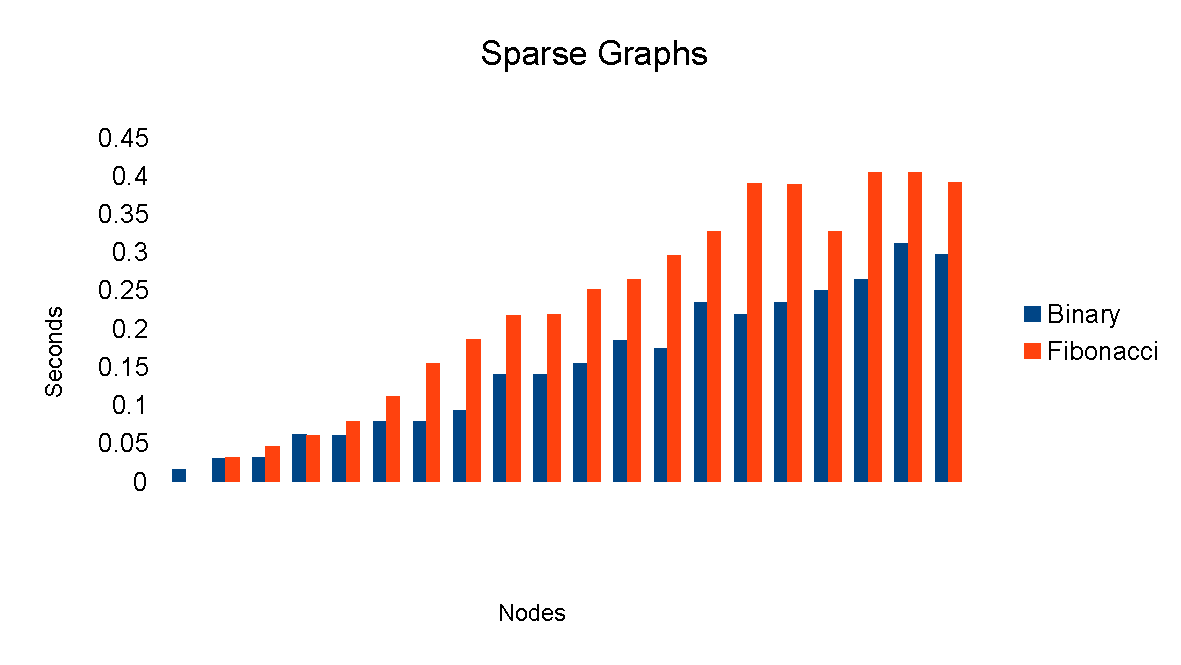
\includegraphics[width=\textwidth]{graphs/sparse}
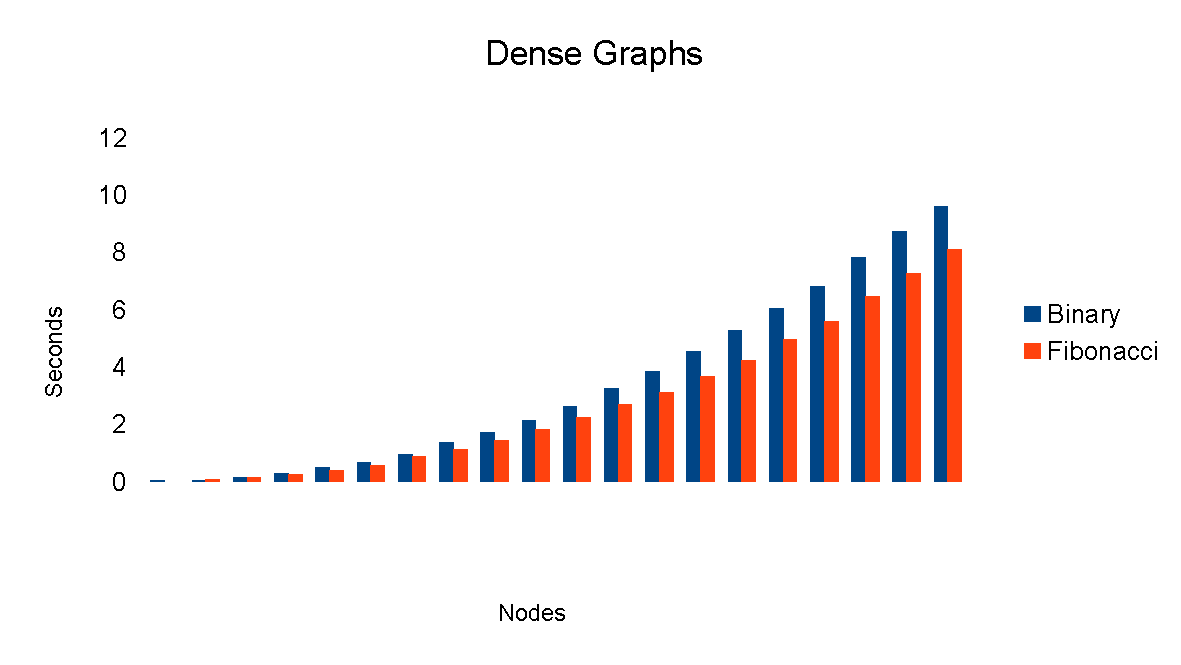
\includegraphics[width=\textwidth]{graphs/dense}

\subsection{Conclusion from the results}

From the results we can see, that the fibonacci heap is slower than the binary heap on the sparse graph, which stems from the slower deletemin in the fibonacci heap, while decreasekey has no effect.

When running on the dense graph, we can see the fibonacci heap growing at a slower pace than the binary heap, since it uses constant time per decreasekey instead of logarithmic.
Even though the running time difference does not appear to be very big on the dense graph, it is actually quite impressing when we look at how heavily binary outperforms fibonacci on the sparse graph. On larger input the running time differences for the sparse graph would have likely favoured fibonacci even more, but unfortunately we did not have the required memory to run much larger data sets.

\subsection{A note on great big data sets}

Actually, it would have been possible to run with much larger data sets, if we had chose to not actually store the neighbour information, but use a weighting function instead. Since the distances between two nodes is fairly predictable, this could have greatly reduced the memory consumption. 